\chapter{Results}
\label{kap:results}

In this chapter, we present results of our trained models, on both training and testing datasets to see how well they generalize.

\section{Inverse rendering}
\subsection{IRN}
We observed that IRN had problems learning normals and view vector much more than other parameters and was only able to learn somewhat meaningful priors only in later stages of training. As complex geometries are used for scenes in our dataset, it did not come as a surprise that IRN had hard time learning normal or view vectors. Other estimated parameters look very similar to ground-truth data, even on test dataset, as shown in figures \ref{fig:irn-train} and \ref{fig:irn-test}.
\begin{figure}[H]
    \centerline{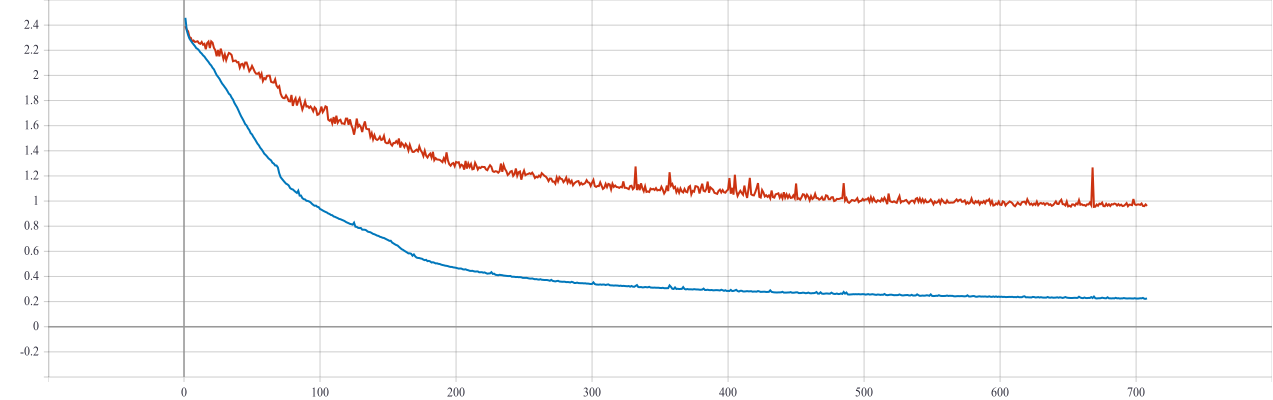
\includegraphics[width=0.6\textwidth]{praca/images/Training-IRN.png}}
    \caption[Training and validation error for IRN]{Training (blue) and validation (red) error during training IRN}
    \label{img:training-irn}
\end{figure}
\begin{figure}
  \centering
  \begin{subfigure}{0.32\linewidth}
    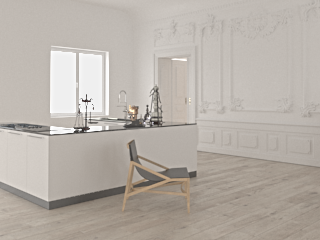
\includegraphics[width=\linewidth]{praca/images/AI43_004_Cam02.png}
    \caption{Original image}
  \end{subfigure}
  \begin{subfigure}{0.32\linewidth}
    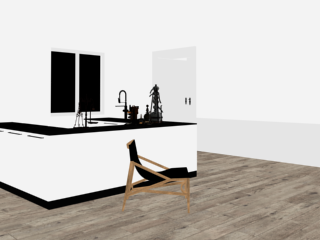
\includegraphics[width=\linewidth]{praca/images/AI43_004_Cam02.albedo.png}
    \caption{GT diffuse albedo}
  \end{subfigure}
  \begin{subfigure}{0.32\linewidth}
    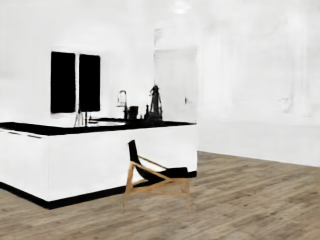
\includegraphics[width=\linewidth]{praca/images/AI43_004_Cam02.albedo_output.png}
    \caption{Predicted diffuse albedo}
  \end{subfigure}
  \begin{subfigure}{0.32\linewidth}
    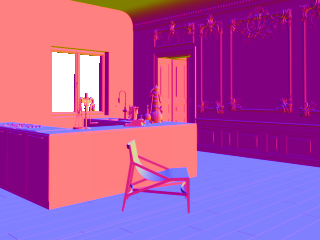
\includegraphics[width=\linewidth]{praca/images/AI43_004_Cam02.normal.png}
    \caption{GT normals}
  \end{subfigure}
  \begin{subfigure}{0.32\linewidth}
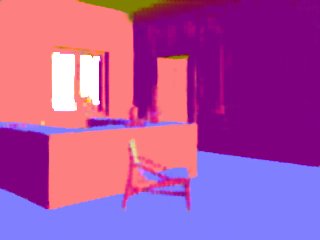
\includegraphics[width=\linewidth]{praca/images/AI43_004_Cam02.normal_output.png}
    \caption{Predicted normals}
  \end{subfigure}
  \begin{subfigure}{0.32\linewidth}
    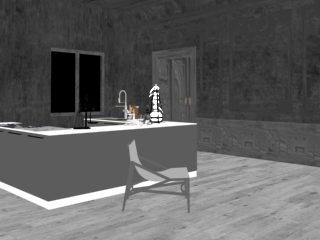
\includegraphics[width=\linewidth]{praca/images/AI43_004_Cam02.specular.png}
    \caption{GT specular albedo}
  \end{subfigure}
  \begin{subfigure}{0.32\linewidth}
    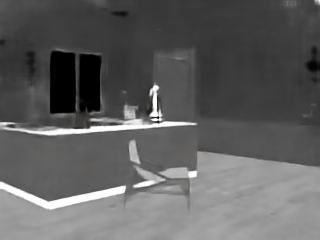
\includegraphics[width=\linewidth]{praca/images/AI43_004_Cam02.specular_output.png}
    \caption{Predicted specular albedo}
  \end{subfigure}
  \begin{subfigure}{0.32\linewidth}
    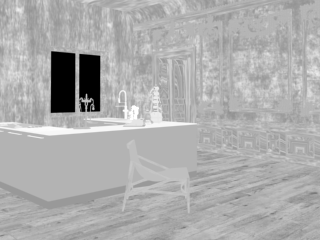
\includegraphics[width=\linewidth]{praca/images/AI43_004_Cam02.glossiness.png}
    \caption{GT glossiness}
  \end{subfigure}
  \begin{subfigure}{0.32\linewidth}
    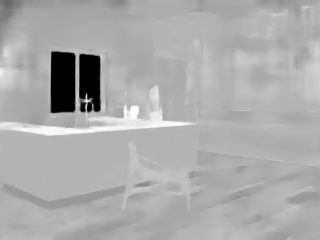
\includegraphics[width=\linewidth]{praca/images/AI43_004_Cam02.glossiness_output.png}
    \caption{Predicted glossiness}
  \end{subfigure}
  \begin{subfigure}{0.32\linewidth}
    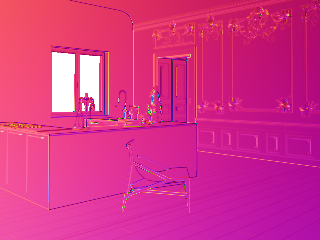
\includegraphics[width=\linewidth]{praca/images/AI43_004_Cam02.view.png}
    \caption{GT view vector}
  \end{subfigure}
  \begin{subfigure}{0.32\linewidth}
    
\includegraphics[width=\linewidth]{praca/images/AI43_004_Cam02.view_output.png}
    \caption{Predicted view vector}
  \end{subfigure}
  \caption[IRN results - train data]{IRN results on train data}
  \label{fig:irn-train}
\end{figure}
\begin{figure}
  \centering
  \begin{subfigure}{0.32\linewidth}
    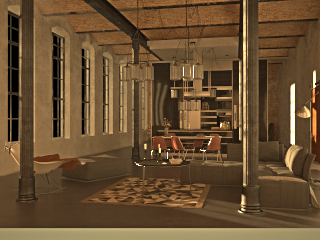
\includegraphics[width=\linewidth]{praca/images/AI46_009_Cam01.VRayLightSelect_RE_L0.png}
    \caption{Original image}
  \end{subfigure}
  \begin{subfigure}{0.32\linewidth}
    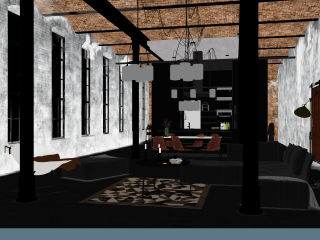
\includegraphics[width=\linewidth]{praca/images/AI46_009_Cam01.VRayLightSelect_RE_L0.albedo.png}
    \caption{GT diffuse albedo}
  \end{subfigure}
  \begin{subfigure}{0.32\linewidth}
    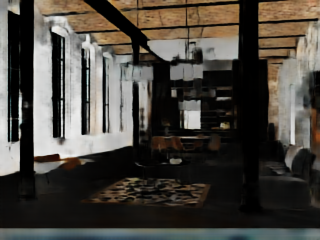
\includegraphics[width=\linewidth]{praca/images/AI46_009_Cam01.VRayLightSelect_RE_L0.albedo_output.png}
    \caption{Predicted diffuse albedo}
  \end{subfigure}
  \begin{subfigure}{0.32\linewidth}
    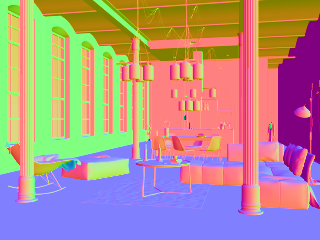
\includegraphics[width=\linewidth]{praca/images/AI46_009_Cam01.VRayLightSelect_RE_L0.normal.png}
    \caption{GT normals}
  \end{subfigure}
  \begin{subfigure}{0.32\linewidth}
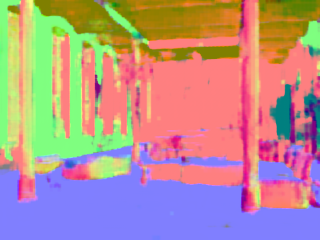
\includegraphics[width=\linewidth]{praca/images/AI46_009_Cam01.VRayLightSelect_RE_L0.normal_output.png}
    \caption{Predicted normals}
  \end{subfigure}
  \begin{subfigure}{0.32\linewidth}
    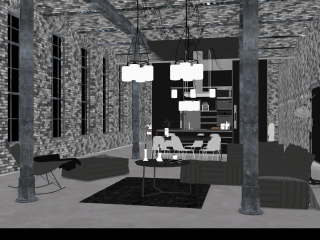
\includegraphics[width=\linewidth]{praca/images/AI46_009_Cam01.VRayLightSelect_RE_L0.specular.png}
    \caption{GT specular albedo}
  \end{subfigure}
  \begin{subfigure}{0.32\linewidth}
    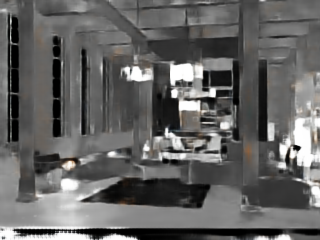
\includegraphics[width=\linewidth]{praca/images/AI46_009_Cam01.VRayLightSelect_RE_L0.specular_output.png}
    \caption{Predicted specular albedo}
  \end{subfigure}
  \begin{subfigure}{0.32\linewidth}
    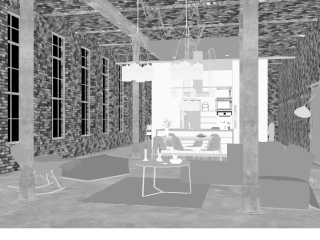
\includegraphics[width=\linewidth]{praca/images/AI46_009_Cam01.VRayLightSelect_RE_L0.glossiness.png}
    \caption{GT glossiness}
  \end{subfigure}
  \begin{subfigure}{0.32\linewidth}
    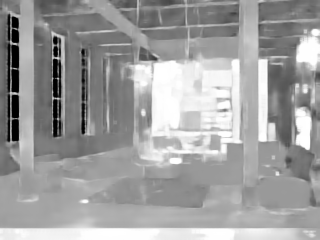
\includegraphics[width=\linewidth]{praca/images/AI46_009_Cam01.VRayLightSelect_RE_L0.glossiness_output.png}
    \caption{Predicted glossiness}
  \end{subfigure}
  \begin{subfigure}{0.32\linewidth}
    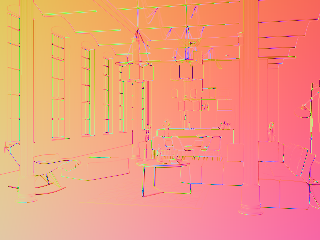
\includegraphics[width=\linewidth]{praca/images/AI46_009_Cam01.VRayLightSelect_RE_L0.view.png}
    \caption{GT view vector}
  \end{subfigure}
  \begin{subfigure}{0.32\linewidth}
    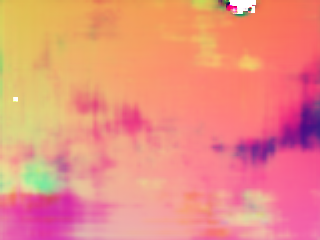
\includegraphics[width=\linewidth]{praca/images/AI46_009_Cam01.VRayLightSelect_RE_L0.view_output.png}
    \caption{Predicted view vector}
  \end{subfigure}
  \caption[IRN results - test data]{IRN results on test data}
  \label{fig:irn-test}
\end{figure}
\subsection{RAR}
Training of RAR net was somewhat successful, as the network was able to learn illumination and shadows that are not present in image computed by direct renderer, even on test dataset, as shown in figures \ref{fig:rar-train} and \ref{fig:rar-test}. But the reconstruction is not perfect, as we have used estimated data from IRN to compute direct image, which already accounts for some error and this error gets amplified even more. We could fix this by train RAR from scratch with direct image being computed from ground-truth data.
\begin{figure}[H]
    \centerline{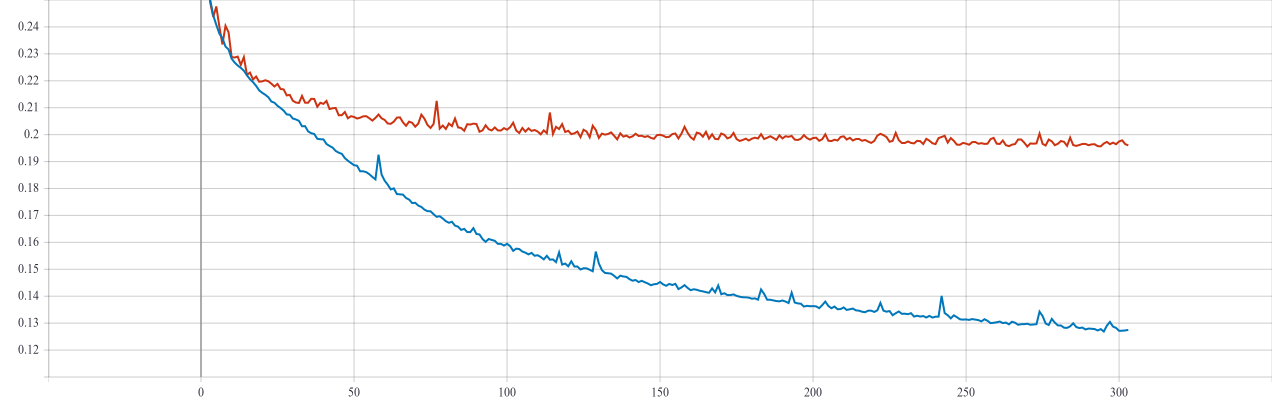
\includegraphics[width=0.6\textwidth]{praca/images/Training-RAR.png}}
    \caption[Training and validation error for RAR]{Training (blue) and validation (red) error during training RAR}
    \label{img:training-rar}
\end{figure}
\begin{figure}[H]
    \centering
    \begin{subfigure}{0.32\linewidth}
        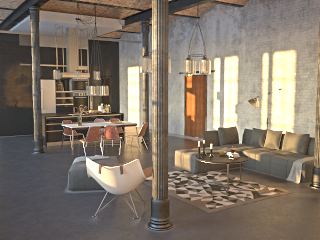
\includegraphics[width=\linewidth]{praca/images/AI46_009_Cam06.png}
        \caption{Original image}
    \end{subfigure}
    \begin{subfigure}{0.32\linewidth}
        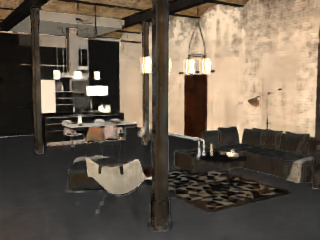
\includegraphics[width=\linewidth]{praca/images/AI46_009_Cam06.direct.png}
        \caption{Direct image}
    \end{subfigure}
    \begin{subfigure}{0.32\linewidth}
        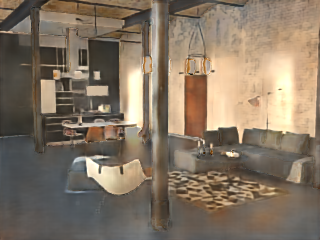
\includegraphics[width=\linewidth]{praca/images/AI46_009_Cam06.reconstructed.png}
        \caption{Reconstructed image}
    \end{subfigure}
    \caption[RAR results - train data]{RAR results on train data}
    \label{fig:rar-train}
\end{figure}
\begin{figure}[H]
    \centering
    \begin{subfigure}{0.32\linewidth}
        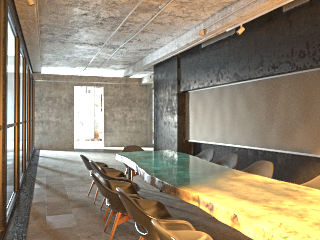
\includegraphics[width=\linewidth]{praca/images/AI47_007_Cam07.VRayLightSelect_RE_L8.png}
        \caption{Original image}
    \end{subfigure}
    \begin{subfigure}{0.32\linewidth}
        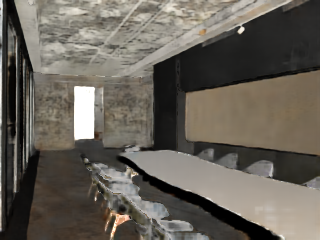
\includegraphics[width=\linewidth]{praca/images/AI47_007_Cam07.VRayLightSelect_RE_L8.direct.png}
        \caption{Direct image}
    \end{subfigure}
    \begin{subfigure}{0.32\linewidth}
        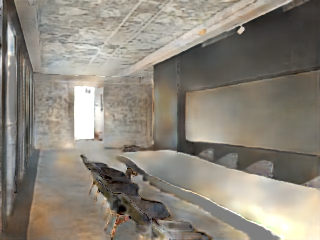
\includegraphics[width=\linewidth]{praca/images/AI47_007_Cam07.VRayLightSelect_RE_L8.reconstructed.png}
        \caption{Reconstructed image}
    \end{subfigure}
    \caption[RAR results - test data]{RAR results on test data}
    \label{fig:rar-test}
\end{figure}
\section{Material Segmentation}
MSN also performed well on both train and test sets, as shown below. Results could be improved by using deeper architecture, as architectures for material segmentation in the past used much more layers, which is also subject for our future work.
\begin{figure}[H]
    \centerline{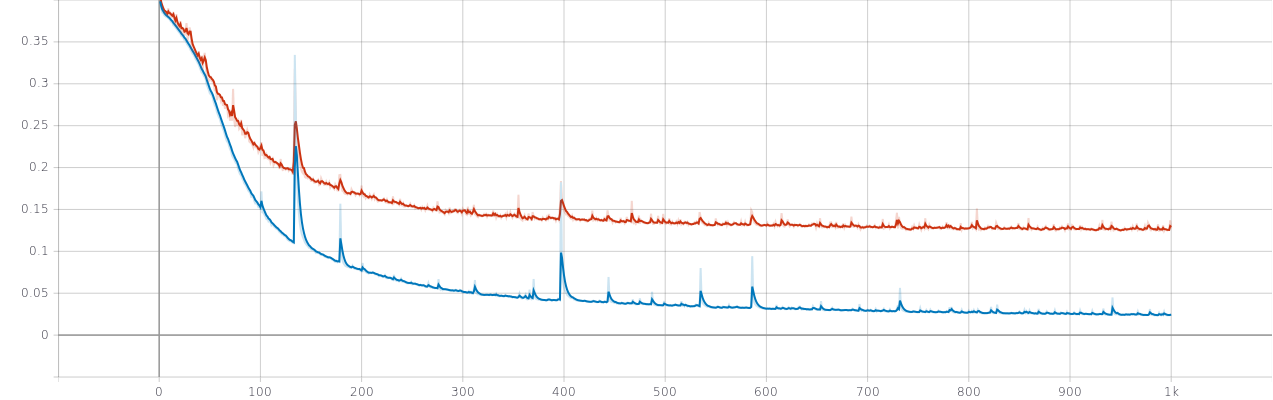
\includegraphics[width=0.6\textwidth]{praca/images/Training-MSN.png}}
    \caption[Training and validation error for MSN]{Training (blue) and validation (red) error during training MSN}
    \label{img:training-msn}
\end{figure}
\begin{figure}[H]
    \centering
    \begin{subfigure}{0.32\linewidth}
        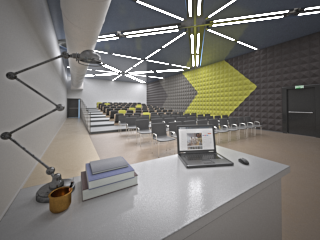
\includegraphics[width=\linewidth]{praca/images/AI53_007_Cam08.png}
        \caption{Original image}
    \end{subfigure}
    \begin{subfigure}{0.32\linewidth}
        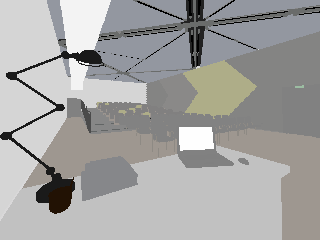
\includegraphics[width=\linewidth]{praca/images/AI53_007_Cam08.segmentation.png}
        \caption{GT segmentation}
    \end{subfigure}
    \begin{subfigure}{0.32\linewidth}
        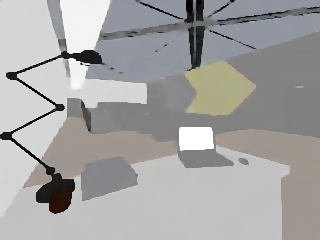
\includegraphics[width=\linewidth]{praca/images/AI53_007_Cam08.predicted_segmentation.png}
        \caption{Predicted segmentation}
    \end{subfigure}
    \caption[MSN results - train data]{MSN results on train data}
    \label{fig:msn-train}
\end{figure}
\begin{figure}[H]
    \centering
    \begin{subfigure}{0.32\linewidth}
        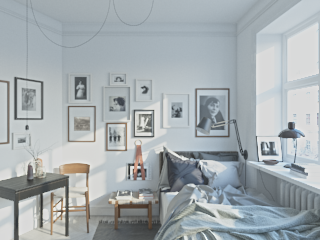
\includegraphics[width=\linewidth]{praca/images/AI45_003_Cam01.png}
        \caption{Original image}
    \end{subfigure}
    \begin{subfigure}{0.32\linewidth}
        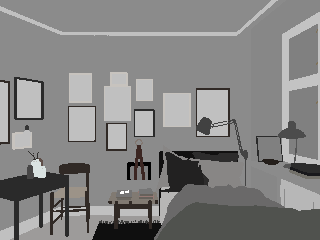
\includegraphics[width=\linewidth]{praca/images/AI45_003_Cam01.segmentation.png}
        \caption{GT segmentation}
    \end{subfigure}
    \begin{subfigure}{0.32\linewidth}
        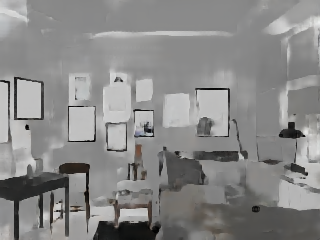
\includegraphics[width=\linewidth]{praca/images/AI45_003_Cam01.predicted_segmentation.png}
        \caption{Predicted segmentation}
    \end{subfigure}
    \caption[MSN results - test data]{MSN results on test data}
    \label{fig:msn-test}
\end{figure}